In this section we informally introduce \lang{} and the concepts needed to combine LIO and FLAM. Section~\ref{sec:calculus} will then formalize the intuitions presented in this section.

Given a named principal $n \in \Nameset$ we call $n$ a \emph{node} when referring to the machine executing code on $n$'s behalf. We assume each named principal has a corresponding machine executing code on its behalf. The node $n$ starts off with a current label $\conf{\bot} \wedge \integ{n}$\footnote{We follow the convention of \cite{Arden:2015:FA:2859845.2859998} and omit projections of the $\bot$ principal} and a clearance label $\conf{n} \wedge \integ{\bot}$. The initial current label represents the fact that no information has been observed by the node, and no information has affected the integrity of the node. The clearance specifies that $n$ can only observe information labeled with a label that flows to $n$, and that $n$'s integrity is allowed to be affected by any other principal.

Figure~\ref{fig:node-info-flow} illustrates running \lang{} with two nodes $n$ and $m$. Node $n$ starts off with a current label $\integ{n}$ and clearance $\conf{n}$, and similarly for $m$. As evaluation proceeds the current label of node $n$ and $m$ will move to the right, but the current label will never enter the white region.

\begin{figure}
    \centering
    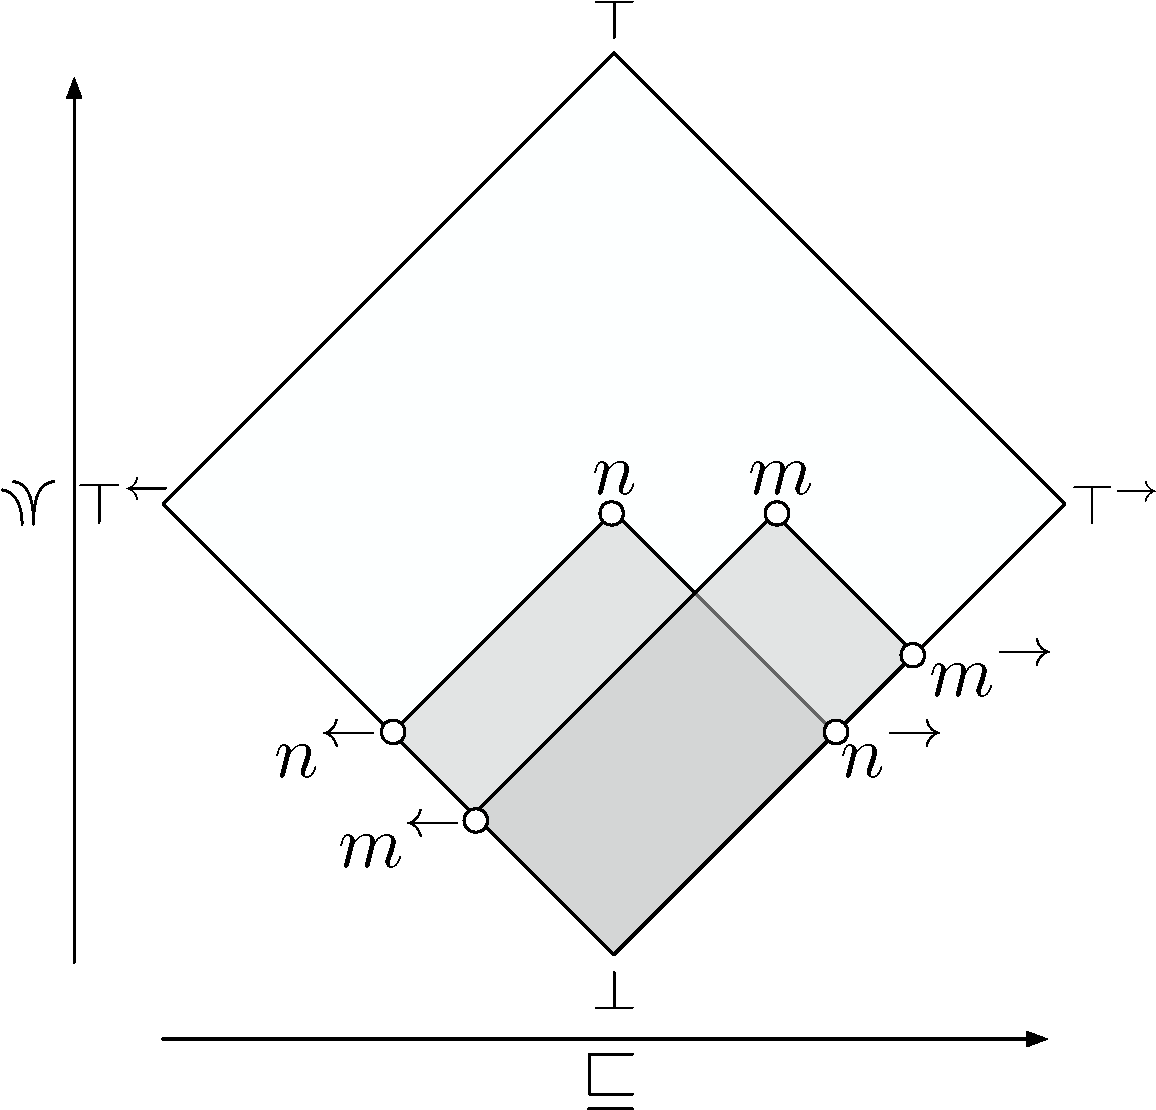
\includegraphics[scale=0.25]{Illustrations/multi-node.pdf}
    \caption{As nodes $n$ and $m$ performs computations their current labels will float from the left-most point to the right-most point in the lattice.}
    \label{fig:node-info-flow}
\end{figure}

\subsection{Remote Procedure Calls}
Nodes in \lang{} communicate by remote invocation of functions on different machines. We annotate functions with the node on which the function should be evaluated. That is, the application $\app{(\abs{n}{p}{x}{\expr})}{\expr'}$ denotes a function $\abs{n}{p}{x}{\expr}$ located on machine $n$ should be evaluated with argument $\expr'$ and the returned expression will be given label $p$. For instance, the expression
\begin{lstlisting}
((*@$\lambda^{n}_{p}$@*) x . not x) b >>= (*@$\lambda^{m}_{m}$@*) y . unlabel y
\end{lstlisting}
computes the negation of the boolean $b$ on node $n$ and returns the result as a labeled value with label $p$, which is then unlabeled on node $m$. After receiving the labeled value computed by node $n$, node $m$ needs to unlabel the value to use it. The unlabel command checks that $p \flowsto \conf{n}$.

\subsection{Proof search}
In order to prove queries of the form $p \flowsto \conf{n}$ a distributed proof search is performed. The two most important rules for the proof search judgment is the rule for using delegations, and the rule for forwarding trust checking to other nodes in the system. We discuss these two rules informally here.

\paragraph{Delegations}
Delegations of the form $\lb{r}{p \actsfor q}$ (pronounced $r$ \emph{says that} $p$ \emph{acts for} $q$) can be used by a proof search on a node $n$ when $r \flowsto \conf{n}$\footnote{The actual judgment requires other trust relationships to hold, but we omit these for now. The rule will be given formally in Section~\ref{sec:calculus}}. We say that the delegation $\lb{r}{p \actsfor q}$ is \emph{labeled} with label $r$. Using a delegation in a proof search will raise the current label by the label of the delegation, and thus fine-grained control of how delegations are used is important. For this reason \lang{} uses \emph{strategies}, which are lists of principals, to specify which delegations can be used in a proof, and in which order. For instance, if the delegation $\lb{r}{p \actsfor q}$ is ``known'' by node $n$ and $n$ is evaluating the expression
\begin{lstlisting}
withStrategy [s, r, t] (p (*@$\actsfor$@*) q)
\end{lstlisting}
the node will first search for the delegations with a label that flows to $s$. Assuming this fails, delegations with a label that flows to $r$ will be used, and if $r \flowsto \conf{n}$ the delegation can be used to complete the proof search. This illustrates how \lang{} performs fine-grained proof search with custom strategies for handling delegations.

\paragraph{Forwarding}
A node $n$ can forward the checking of trust checking to a node $m$ when $n$'s current label flows to $\conf{m}$. Combining uses of this rule with delegations, this allows a node to use delegations local to other nodes in the system. For instance, a server $s$ can represent users authorized by $s$ by delegating ownership projections $\owner{s}{u}$ for every authorized user $u$. The delegation $\lb{\integ{s}}{\owner{s}{u} \actsfor \mathsf{users}}$ then represents that user $u$ is authorized. Another user $u'$ can then evaluate
\begin{lstlisting}
withStrategy [(*@$\integ{s}$@*)] ((*@$\owner{s}{u} \actsfor \mathsf{users}$@*))
\end{lstlisting}
and forward the proof search to the server, which will succeed and return a positive answer back to $u'$.